\documentclass[aspectratio=169, 10pt]{beamer}

% --- Packages ---
\usepackage[utf8]{inputenc}
\usepackage{tikz}
\usepackage{pgfplots}
\usepackage{amsmath, amssymb, amsfonts}
\usepackage{booktabs}
\usepackage{bm}
\usepackage{xcolor}
\usetikzlibrary{arrows.meta, calc, positioning, shapes.geometric, decorations.pathreplacing, backgrounds, fit, shadows, patterns, shapes.arrows, angles, quotes}
\pgfplotsset{compat=1.17}

% NYU Colors
\definecolor{nyupurple}{RGB}{87,46,140}
\definecolor{nyuheader}{RGB}{172,159,195}
\definecolor{nyufooter}{RGB}{189,178,211}

% Theme
\usetheme{default}
\setbeamertemplate{navigation symbols}{}

% Itemize
\setbeamercolor{itemize item}{fg=nyupurple}
\setbeamercolor{itemize subitem}{fg=nyupurple}
\setbeamercolor{itemize subsubitem}{fg=nyupurple}
\setbeamertemplate{itemize item}{\textbullet}
\setbeamertemplate{itemize subitem}{\textbullet}
\setbeamertemplate{itemize subsubitem}{\textbullet}

% Blocks
\setbeamercolor{block title}{fg=white, bg=nyupurple}
\setbeamercolor{block body}{fg=black, bg=nyuheader!30}
\setbeamercolor{block title alerted}{fg=white, bg=red!70}
\setbeamercolor{block body alerted}{fg=black, bg=red!10}
\setbeamercolor{block title example}{fg=white, bg=green!50!black}
\setbeamercolor{block body example}{fg=black, bg=green!10}

% Diagram colors
\definecolor{darkblue}{RGB}{0,51,102}
\definecolor{brightblue}{RGB}{0,102,204}
\definecolor{lightblue}{RGB}{153,204,255}
\definecolor{darkgreen}{RGB}{0,102,51}
\definecolor{accentred}{RGB}{192,0,0}
\definecolor{accentgreen}{RGB}{0,128,0}
\definecolor{accentorange}{RGB}{255,128,0}

% Commands
\newcommand{\vect}[1]{\boldsymbol{#1}}
\newcommand{\mat}[1]{\mathbf{#1}}

% Header
\makeatletter
\setbeamertemplate{frametitle}{%
    \nointerlineskip%
    \begin{beamercolorbox}[wd=\paperwidth,ht=0.7cm,dp=0.15cm,rightskip=0.5cm]{frametitle}
        \hspace{0.3cm}\usebeamerfont{frametitle}\insertframetitle%
        \hfill%
        \raisebox{0.08cm}{{\bfseries\sffamily\color{nyupurple}NYU}}%
    \end{beamercolorbox}%
}
\makeatother
\setbeamercolor{frametitle}{fg=black, bg=nyuheader}
\setbeamerfont{frametitle}{size=\large}

% Footer
\setbeamertemplate{footline}{%
    \begin{tikzpicture}[remember picture, overlay]
        \fill[nyufooter] ([yshift=0.6cm]current page.south west) rectangle ([xshift=5cm]current page.south east);
        \fill[nyufooter!70] ([yshift=0.6cm, xshift=5cm]current page.south west) rectangle ([xshift=10.5cm]current page.south east);
        \fill[nyufooter!40] ([yshift=0.6cm, xshift=10.5cm]current page.south west) rectangle (current page.south east);
        \node[anchor=west, font=\small] at ([xshift=0.3cm, yshift=0.3cm]current page.south west) {Dr.\ Aliasghar Arab};
        \node[anchor=center, font=\small] at ([yshift=0.3cm]current page.south) {Autonomous Mobile Robots};
        \node[anchor=east, font=\small] at ([xshift=-0.3cm, yshift=0.3cm]current page.south east) {LECTURE 3 -- FALL 2025 \quad \insertframenumber{} / \inserttotalframenumber};
    \end{tikzpicture}%
}

% Title page
\defbeamertemplate*{title page}{customized}[1][]
{
    \begin{tikzpicture}[remember picture, overlay]
        \node[anchor=north east] at ([xshift=-0.8cm, yshift=-0.8cm]current page.north east) {%
            {\bfseries\sffamily\Large\color{nyupurple}NYU}%
            {\sffamily\normalsize\color{black}\ \ TANDON SCHOOL OF ENGINEERING}%
        };
    \end{tikzpicture}
    
    \vspace{2cm}
    \centering
    {\Large\bfseries\inserttitle\par}
    \vspace{0.3cm}
    {\insertsubtitle\par}
    \vspace{1cm}
    {\insertauthor\par}
    \vspace{0.3cm}
    {\small\insertinstitute\par}
    \vspace{0.5cm}
    {\insertdate\par}
}

% Title info
\title{Autonomous Mobile Robots}
\subtitle{Lecture 3: Control \& Perception Fundamentals}
\author{Dr.\ Aliasghar Arab}
\institute{NYU Tandon School of Engineering}
\date{Fall 2025}

\begin{document}

% ============================================
% TITLE SLIDE
% ============================================
{
\setbeamertemplate{footline}{}
\begin{frame}[plain]
    \titlepage
\end{frame}
}

% ============================================
% OVERVIEW
% ============================================
\begin{frame}{Lecture Overview}
    \textbf{Today's Topics:}
    
    \vspace{0.4cm}
    \begin{itemize}
        \item Recap: Differential Drive Kinematics
        
        \vspace{0.3cm}
        \item Robot Dynamics via Euler-Lagrange Method
        
        \vspace{0.3cm}
        \item Example: One-Wheeled Balancing Robot
        
        \vspace{0.3cm}
        \item Perception Fundamentals
        
        \vspace{0.3cm}
        \item Coupled Vehicle-Manipulator Systems
        
        \vspace{0.3cm}
        \item Coordinate Transformations \& Swerve Drive
    \end{itemize}
\end{frame}

% ============================================
% COURSE TOPICS
% ============================================
\begin{frame}{Course Topics}
    \begin{enumerate}
        \item Introduction \& Physical Constraints
        
        \vspace{0.2cm}
        \item Vehicle Kinematics \& Equations of Motion
        
        \vspace{0.2cm}
        \item[\textcolor{accentred}{\textbf{3.}}] \textcolor{accentred}{\textbf{Control \& Perception Fundamentals}}
        
        \vspace{0.2cm}
        \item Nonlinear Control Methods
        
        \vspace{0.2cm}
        \item Advanced Model Predictive Control (NMPC) + Constraints
        
        \vspace{0.2cm}
        \item Motion Planning Algorithms (RRT*, RRT, DWA)
        
        \vspace{0.2cm}
        \item Learning-Based Planning \& Control
        
        \vspace{0.2cm}
        \item Industry Standards, Architectures, \& Safety
    \end{enumerate}
\end{frame}

% ============================================
% PART I: KINEMATICS RECAP
% ============================================
\begin{frame}{}
    \vfill
    \centering
    {\Large\textbf{Part I}}
    
    \vspace{0.5cm}
    {\large Differential Drive Kinematics Recap}
    \vfill
\end{frame}

% ============================================
% DIFFERENTIAL DRIVE - CONFIGURATION
% ============================================
\begin{frame}{Differential Drive Robot: Configuration}
    \begin{columns}[T]
        \begin{column}{0.48\textwidth}
            \textbf{Physical Parameters:}
            
            \vspace{0.3cm}
            \begin{itemize}
                \item Two wheels with radius $r$
                
                \vspace{0.3cm}
                \item Distance between wheels: $2b$
                
                \vspace{0.3cm}
                \item Wheel angular velocities:
                \begin{itemize}
                    \item $\dot{\phi}_1$ (right wheel)
                    \item $\dot{\phi}_2$ (left wheel)
                \end{itemize}
            \end{itemize}
        \end{column}
        \begin{column}{0.48\textwidth}
            \centering
            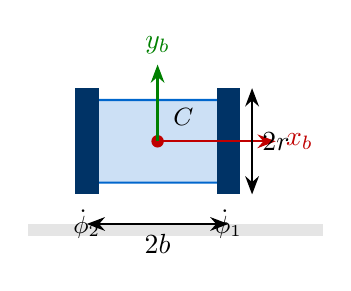
\begin{tikzpicture}[scale=0.75, >=Stealth]
                % Ground
                \fill[gray!20] (-2.2,-1.6) rectangle (2.8,-1.4);
                
                % Robot body (top view)
                \fill[brightblue!20, draw=brightblue, thick, rounded corners=3pt] 
                    (-1.2,-0.7) rectangle (1.2,0.7);
                
                % Wheels
                \fill[darkblue] (-1.4,-0.9) rectangle (-1.0,0.9);
                \fill[darkblue] (1.0,-0.9) rectangle (1.4,0.9);
                
                % Wheel labels
                \node[below, font=\small] at (-1.2,-1.0) {$\dot{\phi}_2$};
                \node[below, font=\small] at (1.2,-1.0) {$\dot{\phi}_1$};
                
                % Center point
                \fill[accentred] (0,0) circle (3pt);
                \node[above right, font=\small] at (0.1,0.1) {$C$};
                
                % Body frame axes
                \draw[->, thick, accentred] (0,0) -- (2,0) node[right] {$x_b$};
                \draw[->, thick, accentgreen] (0,0) -- (0,1.3) node[above] {$y_b$};
                
                % Dimension: 2b
                \draw[<->, thick] (-1.2,-1.4) -- (1.2,-1.4) node[midway, below] {$2b$};
                
                % Dimension: r
                \draw[<->, thick] (1.6,-0.9) -- (1.6,0.9) node[midway, right] {$2r$};
            \end{tikzpicture}
        \end{column}
    \end{columns}
\end{frame}

% ============================================
% DIFFERENTIAL DRIVE - VELOCITIES
% ============================================
\begin{frame}{Differential Drive: Body Velocities}
    \textbf{From wheel speeds to body velocities:}
    
    \vspace{0.4cm}
    \begin{columns}[T]
        \begin{column}{0.45\textwidth}
            \textbf{Linear velocity} (forward):
            \[
            \boxed{v_x = \frac{r}{2}\left(\dot{\phi}_1 + \dot{\phi}_2\right)}
            \]
            
            \vspace{0.4cm}
            \textbf{Angular velocity} (yaw rate):
            \[
            \boxed{\omega = \frac{r}{2b}\left(\dot{\phi}_1 - \dot{\phi}_2\right)}
            \]
        \end{column}
        \begin{column}{0.5\textwidth}
            \centering
            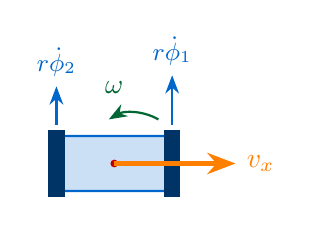
\begin{tikzpicture}[scale=0.7, >=Stealth]
                % Robot body
                \fill[brightblue!20, draw=brightblue, thick, rounded corners=2pt] 
                    (-1,-0.5) rectangle (1,0.5);
                
                % Wheels
                \fill[darkblue] (-1.2,-0.6) rectangle (-0.9,0.6);
                \fill[darkblue] (0.9,-0.6) rectangle (1.2,0.6);
                
                % Center
                \fill[accentred] (0,0) circle (2pt);
                
                % Forward velocity
                \draw[->, ultra thick, accentorange] (0,0) -- (2.2,0) node[right] {$v_x$};
                
                % Angular velocity
                \draw[->, thick, darkgreen] (0.8,0.8) arc (60:120:0.9);
                \node[darkgreen, above] at (0,1.1) {$\omega$};
                
                % Wheel velocities
                \draw[->, thick, brightblue] (-1.05,0.7) -- (-1.05,1.4) node[above, font=\small] {$r\dot{\phi}_2$};
                \draw[->, thick, brightblue] (1.05,0.7) -- (1.05,1.6) node[above, font=\small] {$r\dot{\phi}_1$};
            \end{tikzpicture}
        \end{column}
    \end{columns}
    
    \vspace{0.5cm}
    \begin{block}{Nonholonomic Constraint}
        Lateral velocity is always zero: $v_y = 0$ (robot cannot move sideways)
    \end{block}
\end{frame}

% ============================================
% STATE-SPACE KINEMATICS
% ============================================
\begin{frame}{State-Space Kinematics}
    \textbf{Robot pose in global frame:}
    \[
    \vect{X} = \begin{bmatrix} x \\ y \\ \theta \end{bmatrix}
    \]
    
    \vspace{0.3cm}
    \textbf{Motion equations:}
    \[
    \begin{bmatrix} \dot{x} \\ \dot{y} \\ \dot{\theta} \end{bmatrix} = 
    \begin{bmatrix} \cos\theta & 0 \\ \sin\theta & 0 \\ 0 & 1 \end{bmatrix}
    \begin{bmatrix} v \\ \omega \end{bmatrix}
    \]
    
    \vspace{0.3cm}
    \textbf{Compact form:}
    \[
    \boxed{\dot{\vect{x}} = f(\vect{x}, \vect{u})}
    \]
    
    \vspace{0.2cm}
    where $\vect{u} = [v, \omega]^T$ is the control input.
\end{frame}

% ============================================
% STATE-SPACE DIAGRAM
% ============================================
\begin{frame}{State-Space Kinematics: Visualization}
    \centering
    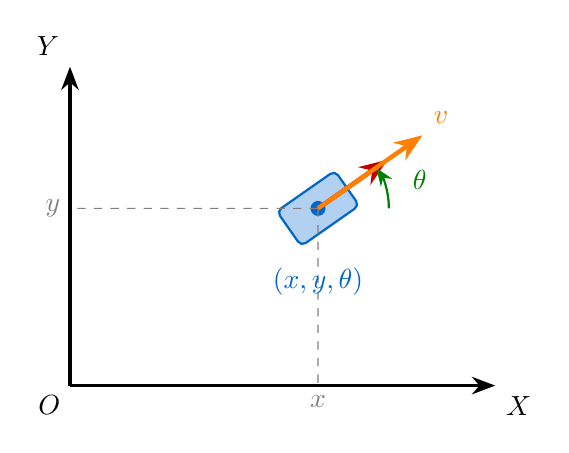
\begin{tikzpicture}[scale=0.9, >=Stealth]
        % Global frame
        \draw[->, very thick] (0,0) -- (6,0) node[below right] {$X$};
        \draw[->, very thick] (0,0) -- (0,4.5) node[above left] {$Y$};
        \node[below left] at (0,0) {$O$};
        
        % Robot position
        \coordinate (robot) at (3.5, 2.5);
        
        % Robot body
        \begin{scope}[shift={(robot)}, rotate=35]
            \fill[brightblue!30, draw=brightblue, thick, rounded corners=2pt] 
                (-0.5,-0.3) rectangle (0.5,0.3);
            \draw[->, ultra thick, accentred] (0,0) -- (1.2,0);
            \fill[brightblue] (0,0) circle (3pt);
        \end{scope}
        
        % Position coordinates
        \draw[dashed, gray] (robot) -- (3.5,0) node[below] {$x$};
        \draw[dashed, gray] (robot) -- (0,2.5) node[left] {$y$};
        
        % Angle theta
        \draw[->, thick, accentgreen] (4.5,2.5) arc (0:35:1);
        \node[accentgreen, right] at (4.7,2.9) {$\theta$};
        
        % Velocity vector
        \draw[->, ultra thick, accentorange] (robot) -- ++(35:1.8) node[above right] {$v$};
        
        % Labels
        \node[below, brightblue] at (3.5,1.8) {$(x, y, \theta)$};
    \end{tikzpicture}
\end{frame}

% ============================================
% PART II: DYNAMICS
% ============================================
\begin{frame}{}
    \vfill
    \centering
    {\Large\textbf{Part II}}
    
    \vspace{0.5cm}
    {\large Robot Dynamics}
    \vfill
\end{frame}

% ============================================
% GENERAL EOM
% ============================================
\begin{frame}{Dynamics: General Equations of Motion}
    \textbf{General dynamic model:}
    \[
    \boxed{\mat{M}(\vect{q})\ddot{\vect{q}} + \mat{C}(\vect{q}, \dot{\vect{q}})\dot{\vect{q}} + \vect{G}(\vect{q}) = \mat{B}_x(\vect{q})\vect{F}_x + \mat{B}_y\vect{F}_y}
    \]
    
    \vspace{0.5cm}
    \begin{columns}[T]
        \begin{column}{0.48\textwidth}
            \begin{itemize}
                \item $\mat{M}(\vect{q})$: Mass/inertia matrix
                
                \vspace{0.3cm}
                \item $\mat{C}(\vect{q}, \dot{\vect{q}})$: Coriolis/centrifugal
                
                \vspace{0.3cm}
                \item $\vect{G}(\vect{q})$: Gravity terms
            \end{itemize}
        \end{column}
        \begin{column}{0.48\textwidth}
            \begin{itemize}
                \item $\mat{B}_x, \mat{B}_y$: Input mappings
                
                \vspace{0.3cm}
                \item $\vect{F}_x, \vect{F}_y$: Wheel forces
                
                \vspace{0.3cm}
                \item $\vect{q}$: Generalized coordinates
            \end{itemize}
        \end{column}
    \end{columns}
\end{frame}

% ============================================
% ASSUMPTIONS
% ============================================
\begin{frame}{Fundamental Assumptions}
    \begin{columns}[T]
        \begin{column}{0.55\textwidth}
            \textbf{No Slipping (Longitudinal):}
            \[
            r\dot{\phi} = V_{wx}
            \]
            Wheel rolls without slipping in direction of motion.
            
            \vspace{0.5cm}
            \textbf{No Sliding (Lateral):}
            \[
            V_{wy} = 0 \quad \Rightarrow \quad F_y = 0
            \]
            No sideways velocity at wheel contact.
        \end{column}
        \begin{column}{0.42\textwidth}
            \centering
            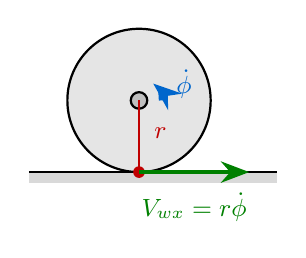
\begin{tikzpicture}[scale=0.7, >=Stealth]
                % Wheel (side view)
                \draw[thick, fill=gray!20] (0,0) circle (1.3);
                \draw[thick, fill=gray!50] (0,0) circle (0.15);
                
                % Radius
                \draw[thick, accentred] (0,0) -- (0,-1.3);
                \node[accentred, right, font=\small] at (0.1,-0.6) {$r$};
                
                % Angular velocity
                \draw[->, ultra thick, brightblue] (0.4,0) arc (0:50:0.4);
                \node[brightblue, right, font=\small] at (0.5,0.3) {$\dot{\phi}$};
                
                % Ground
                \fill[gray!30] (-2,-1.5) rectangle (2.5,-1.3);
                \draw[thick] (-2,-1.3) -- (2.5,-1.3);
                
                % Contact point
                \fill[accentred] (0,-1.3) circle (3pt);
                
                % Velocity at contact
                \draw[->, ultra thick, accentgreen] (0,-1.3) -- (2,-1.3);
                \node[accentgreen, below, font=\small] at (1,-1.5) {$V_{wx} = r\dot{\phi}$};
            \end{tikzpicture}
        \end{column}
    \end{columns}
\end{frame}

% ============================================
% PART III: BALANCING ROBOT
% ============================================
\begin{frame}{}
    \vfill
    \centering
    {\Large\textbf{Part III}}
    
    \vspace{0.5cm}
    {\large One-Wheeled Balancing Robot}
    
    \vspace{0.3cm}
    {\small Euler-Lagrange Derivation}
    \vfill
\end{frame}

% ============================================
% BALANCING ROBOT CONFIG
% ============================================
\begin{frame}{One-Wheeled Balancing Robot: Configuration}
    \begin{columns}[T]
        \begin{column}{0.45\textwidth}
            \textbf{System Parameters:}
            
            \vspace{0.3cm}
            \begin{itemize}
                \item Wheel radius: $r$
                
                \vspace{0.3cm}
                \item Body length: $L$
                
                \vspace{0.3cm}
                \item Total mass: $m$
            \end{itemize}
            
            \vspace{0.4cm}
            \textbf{Generalized Coordinates:}
            
            \vspace{0.3cm}
            \begin{itemize}
                \item $\phi$: Wheel angle
                
                \vspace{0.3cm}
                \item $\theta$: Body tilt from vertical
            \end{itemize}
        \end{column}
        \begin{column}{0.52\textwidth}
            \centering
            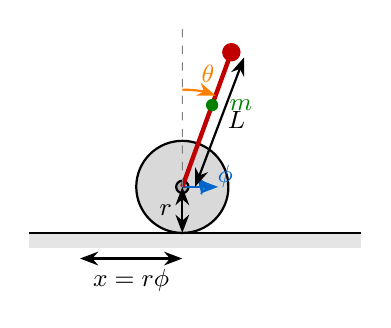
\begin{tikzpicture}[scale=0.65, >=Stealth]
                % Ground
                \fill[gray!20] (-1,-0.3) rectangle (5.5,0);
                \draw[thick] (-1,0) -- (5.5,0);
                
                % Wheel
                \draw[thick, fill=gray!30] (2,0.9) circle (0.9);
                \draw[thick, fill=gray!60] (2,0.9) circle (0.12);
                
                % Wheel angle arc
                \draw[->, thick, brightblue] (2,0.9) -- (2.7,0.9);
                \draw[->, thick, brightblue] (2.35,0.9) arc (0:35:0.35);
                \node[brightblue, right, font=\small] at (2.5,1.1) {$\phi$};
                
                % Body (tilted pendulum)
                \coordinate (wheelcenter) at (2, 0.9);
                \coordinate (bodytop) at ($(wheelcenter) + (70:2.8)$);
                
                % Body
                \draw[ultra thick, accentred] (wheelcenter) -- (bodytop);
                \fill[accentred] (bodytop) circle (0.18);
                
                % Center of mass
                \coordinate (com) at ($(wheelcenter) + (70:1.7)$);
                \fill[accentgreen] (com) circle (0.12);
                \node[accentgreen, right, font=\small] at ($(com) + (0.15,0)$) {$m$};
                
                % Vertical reference
                \draw[dashed, gray] (wheelcenter) -- (2,4);
                
                % Theta angle
                \draw[->, thick, accentorange] (2,2.8) arc (90:70:1.9);
                \node[accentorange, font=\small] at (2.5,3.1) {$\theta$};
                
                % Dimensions
                \draw[<->, thick] (2,0) -- (2,0.9) node[midway, left, font=\small] {$r$};
                \draw[<->, thick] ($(wheelcenter) + (0.25,0)$) -- ($(bodytop) + (0.25,-0.1)$);
                \node[right, font=\small] at ($(wheelcenter) + (0.7,1.3)$) {$L$};
                
                % Ground position
                \draw[<->, thick] (0,-0.5) -- (2,-0.5) node[midway, below, font=\small] {$x = r\phi$};
            \end{tikzpicture}
        \end{column}
    \end{columns}
\end{frame}

% ============================================
% POSITION RELATIONS
% ============================================
\begin{frame}{Position Relations}
    \textbf{Wheel position:}
    \[
    x = r\phi
    \]
    
    \vspace{0.4cm}
    \textbf{Center of mass position:}
    
    \vspace{0.3cm}
    \begin{columns}[T]
        \begin{column}{0.45\textwidth}
            Horizontal:
            \[
            \boxed{x_c = x + L\sin\theta = r\phi + L\sin\theta}
            \]
        \end{column}
        \begin{column}{0.45\textwidth}
            Vertical:
            \[
            \boxed{z_c = L\cos\theta + r}
            \]
        \end{column}
    \end{columns}
    
    \vspace{0.5cm}
    \textbf{Velocities:}
    \[
    \dot{x}_c = r\dot{\phi} + L\dot{\theta}\cos\theta
    \]
    \[
    \dot{z}_c = -L\dot{\theta}\sin\theta
    \]
\end{frame}

% ============================================
% KINETIC ENERGY
% ============================================
\begin{frame}{Kinetic Energy}
    \textbf{Total kinetic energy:}
    \[
    K = \underbrace{\frac{1}{2}m\left(\dot{x}_c^2 + \dot{z}_c^2\right)}_{\text{translational}} + \underbrace{\frac{1}{2}I_w\dot{\phi}^2}_{\text{wheel rotation}} + \underbrace{\frac{1}{2}I_b\dot{\theta}^2}_{\text{body rotation}}
    \]
    
    \vspace{0.4cm}
    \textbf{Substituting velocity expressions:}
    
    \vspace{0.3cm}
    \[
    \dot{x}_c^2 = \left(r\dot{\phi} + L\dot{\theta}\cos\theta\right)^2
    \]
    
    \vspace{0.2cm}
    \[
    \dot{z}_c^2 = L^2\dot{\theta}^2\sin^2\theta
    \]
    
    \vspace{0.3cm}
    \[
    \dot{x}_c^2 + \dot{z}_c^2 = r^2\dot{\phi}^2 + 2rL\dot{\phi}\dot{\theta}\cos\theta + L^2\dot{\theta}^2
    \]
\end{frame}

% ============================================
% POTENTIAL ENERGY
% ============================================
\begin{frame}{Potential Energy \& Lagrangian}
    \textbf{Potential energy:}
    \[
    V = mgz_c = mg(r + L\cos\theta)
    \]
    
    \vspace{0.3cm}
    Taking reference at $\theta = 0$ (upright):
    \[
    \boxed{V = mgL(\cos\theta - 1)}
    \]
    
    \vspace{0.5cm}
    \textbf{Lagrangian:}
    \[
    \boxed{\mathcal{L} = K - V}
    \]
    
    \vspace{0.3cm}
    \begin{block}{Euler-Lagrange Equation}
        For each generalized coordinate $q_i$:
        \[
        \frac{d}{dt}\left(\frac{\partial \mathcal{L}}{\partial \dot{q}_i}\right) - \frac{\partial \mathcal{L}}{\partial q_i} = Q_i
        \]
    \end{block}
\end{frame}

% ============================================
% EL FOR PHI - PART 1
% ============================================
\begin{frame}{Euler-Lagrange for $\phi$: Computing Derivatives}
    \textbf{Step 1:} Compute $\frac{\partial \mathcal{L}}{\partial \dot{\phi}}$
    
    \vspace{0.4cm}
    \[
    \frac{\partial \mathcal{L}}{\partial \dot{\phi}} = mr^2\dot{\phi} + mrL\dot{\theta}\cos\theta + I_w\dot{\phi}
    \]
    
    \vspace{0.5cm}
    \textbf{Step 2:} Compute time derivative
    
    \vspace{0.3cm}
    \[
    \frac{d}{dt}\left(\frac{\partial \mathcal{L}}{\partial \dot{\phi}}\right) = (mr^2 + I_w)\ddot{\phi} + mrL\ddot{\theta}\cos\theta - mrL\dot{\theta}^2\sin\theta
    \]
    
    \vspace{0.5cm}
    \textbf{Step 3:} $\frac{\partial \mathcal{L}}{\partial \phi} = 0$ (no explicit $\phi$ dependence)
\end{frame}

% ============================================
% EL FOR PHI - PART 2
% ============================================
\begin{frame}{Euler-Lagrange for $\phi$: First EOM}
    \textbf{Euler-Lagrange equation:}
    \[
    \frac{d}{dt}\left(\frac{\partial \mathcal{L}}{\partial \dot{\phi}}\right) - \frac{\partial \mathcal{L}}{\partial \phi} = \tau
    \]
    
    \vspace{0.5cm}
    \textbf{First Equation of Motion (EOM-1):}
    \[
    \boxed{(mr^2 + I_w)\ddot{\phi} + mrL\cos\theta\,\ddot{\theta} - mrL\sin\theta\,\dot{\theta}^2 = \tau}
    \]
    
    \vspace{0.4cm}
    where $\tau$ is the motor torque applied to the wheel.
\end{frame}

% ============================================
% EL FOR THETA - PART 1
% ============================================
\begin{frame}{Euler-Lagrange for $\theta$: Computing Derivatives}
    \textbf{Step 1:} Compute $\frac{\partial \mathcal{L}}{\partial \dot{\theta}}$
    
    \vspace{0.4cm}
    \[
    \frac{\partial \mathcal{L}}{\partial \dot{\theta}} = mL^2\dot{\theta} + mrL\dot{\phi}\cos\theta + I_b\dot{\theta}
    \]
    
    \vspace{0.5cm}
    \textbf{Step 2:} Time derivative
    
    \vspace{0.3cm}
    \[
    \frac{d}{dt}\left(\frac{\partial \mathcal{L}}{\partial \dot{\theta}}\right) = (mL^2 + I_b)\ddot{\theta} + mrL\ddot{\phi}\cos\theta - mrL\dot{\phi}\dot{\theta}\sin\theta
    \]
    
    \vspace{0.5cm}
    \textbf{Step 3:} Compute $\frac{\partial \mathcal{L}}{\partial \theta}$
    
    \vspace{0.3cm}
    \[
    \frac{\partial \mathcal{L}}{\partial \theta} = -mrL\dot{\phi}\dot{\theta}\sin\theta + mgL\sin\theta
    \]
\end{frame}

% ============================================
% EL FOR THETA - PART 2
% ============================================
\begin{frame}{Euler-Lagrange for $\theta$: Second EOM}
    \textbf{Euler-Lagrange equation:}
    \[
    \frac{d}{dt}\left(\frac{\partial \mathcal{L}}{\partial \dot{\theta}}\right) - \frac{\partial \mathcal{L}}{\partial \theta} = 0
    \]
    
    \vspace{0.4cm}
    (No external torque on $\theta$ --- only gravity acts)
    
    \vspace{0.5cm}
    \textbf{Second Equation of Motion (EOM-2):}
    \[
    \boxed{(mL^2 + I_b)\ddot{\theta} + mrL\cos\theta\,\ddot{\phi} - mgL\sin\theta = 0}
    \]
\end{frame}

% ============================================
% MATRIX FORM
% ============================================
\begin{frame}{Equations in Matrix Form}
    \textbf{Standard form:} $\mat{M}(\vect{q})\ddot{\vect{q}} + \mat{C}(\vect{q},\dot{\vect{q}})\dot{\vect{q}} + \vect{G}(\vect{q}) = \vect{\tau}$
    
    \vspace{0.4cm}
    \textbf{Mass Matrix:}
    \[
    \mat{M}(\theta) = \begin{bmatrix} mr^2 + I_w & mrL\cos\theta \\ mrL\cos\theta & mL^2 + I_b \end{bmatrix}
    \]
    
    \vspace{0.4cm}
    \textbf{Coriolis Matrix:}
    \[
    \mat{C}(\theta, \dot{\theta}) = \begin{bmatrix} 0 & -mrL\sin\theta\,\dot{\theta} \\ 0 & 0 \end{bmatrix}
    \]
\end{frame}

% ============================================
% MATRIX FORM - CONTINUED
% ============================================
\begin{frame}{Equations in Matrix Form (continued)}
    \textbf{Gravity Vector:}
    \[
    \vect{G}(\theta) = \begin{bmatrix} 0 \\ -mgL\sin\theta \end{bmatrix}
    \]
    
    \vspace{0.4cm}
    \textbf{Input Vector:}
    \[
    \vect{\tau} = \begin{bmatrix} \tau \\ 0 \end{bmatrix}
    \]
    
    \vspace{0.4cm}
    \textbf{Complete Dynamic Equation:}
    \[
    \boxed{
    \begin{bmatrix} mr^2 + I_w & mrL\cos\theta \\ mrL\cos\theta & mL^2 + I_b \end{bmatrix}
    \begin{bmatrix} \ddot{\phi} \\ \ddot{\theta} \end{bmatrix}
    +
    \begin{bmatrix} -mrL\sin\theta\,\dot{\theta}^2 \\ -mgL\sin\theta \end{bmatrix}
    =
    \begin{bmatrix} \tau \\ 0 \end{bmatrix}
    }
    \]
\end{frame}

% ============================================
% MATRIX PROPERTIES
% ============================================
\begin{frame}{Matrix Properties}
    \begin{block}{Key Properties}
        \begin{itemize}
            \item $\mat{M}(\theta)$ is symmetric and positive definite
            
            \vspace{0.3cm}
            \item Coupling through off-diagonal term $mrL\cos\theta$
            
            \vspace{0.3cm}
            \item Equilibrium at $\theta = 0$ is \textbf{unstable}
        \end{itemize}
    \end{block}
    
    \vspace{0.5cm}
    \begin{alertblock}{Control Objective}
        Design torque $\tau$ to:
        \begin{itemize}
            \item Stabilize body upright: $\theta \to 0$
            \item Control position: $x = r\phi \to x_{\text{desired}}$
        \end{itemize}
    \end{alertblock}
\end{frame}

% ============================================
% PART IV: PERCEPTION
% ============================================
\begin{frame}{}
    \vfill
    \centering
    {\Large\textbf{Part IV}}
    
    \vspace{0.5cm}
    {\large Perception Fundamentals}
    \vfill
\end{frame}

% ============================================
% WHY PERCEPTION
% ============================================
\begin{frame}{Why Perception?}
    \textbf{The Problem:}
    
    \vspace{0.4cm}
    \begin{itemize}
        \item Dynamics give us motion equations
        
        \vspace{0.3cm}
        \item But we need to know where the robot \textbf{actually is}
        
        \vspace{0.3cm}
        \item Sensors are noisy and imperfect
    \end{itemize}
    
    \vspace{0.5cm}
    \begin{block}{Definition}
        \textbf{Perception} is the process of estimating the robot's pose (position and orientation) relative to the world using sensor measurements.
    \end{block}
\end{frame}

% ============================================
% PERCEPTION ERRORS
% ============================================
\begin{frame}{Perception Errors}
    \begin{columns}[T]
        \begin{column}{0.5\textwidth}
            \textbf{Error Components:}
            \[
            \vect{e} = \vect{X}_{\text{true}} - \vect{X}_{\text{measured}}
            \]
            
            \vspace{0.3cm}
            \[
            \vect{e} = \begin{bmatrix} e_x \\ e_y \\ e_\theta \end{bmatrix}
            \]
            
            \vspace{0.4cm}
            \textbf{Error Sources:}
            \begin{itemize}
                \item Sensor noise
                \item Sensor bias
                \item Drift over time
            \end{itemize}
        \end{column}
        \begin{column}{0.47\textwidth}
            \centering
            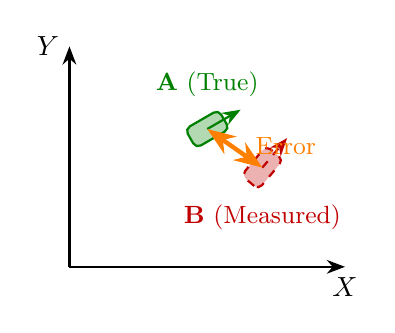
\begin{tikzpicture}[scale=0.7, >=Stealth]
                % Axes
                \draw[->, thick] (0,0) -- (5,0) node[below] {$X$};
                \draw[->, thick] (0,0) -- (0,4) node[left] {$Y$};
                
                % True position A
                \coordinate (A) at (2.5,2.5);
                \begin{scope}[shift={(A)}, rotate=30]
                    \fill[accentgreen!30, draw=accentgreen, thick, rounded corners=2pt] 
                        (-0.35,-0.2) rectangle (0.35,0.2);
                    \draw[->, thick, accentgreen] (0,0) -- (0.7,0);
                \end{scope}
                \node[accentgreen, above, font=\small] at (2.5,2.9) {\textbf{A} (True)};
                
                % Measured position B
                \coordinate (B) at (3.5,1.8);
                \begin{scope}[shift={(B)}, rotate=50]
                    \fill[accentred!30, draw=accentred, thick, rounded corners=2pt, dashed] 
                        (-0.35,-0.2) rectangle (0.35,0.2);
                    \draw[->, thick, accentred, dashed] (0,0) -- (0.7,0);
                \end{scope}
                \node[accentred, below, font=\small] at (3.5,1.3) {\textbf{B} (Measured)};
                
                % Error arrow
                \draw[<->, ultra thick, accentorange] (A) -- (B);
                \node[accentorange, right, font=\small] at (3.2,2.2) {Error};
            \end{tikzpicture}
        \end{column}
    \end{columns}
\end{frame}

% ============================================
% SENSORS FOR LOCALIZATION
% ============================================
\begin{frame}{Sensing for Localization}
    \centering
    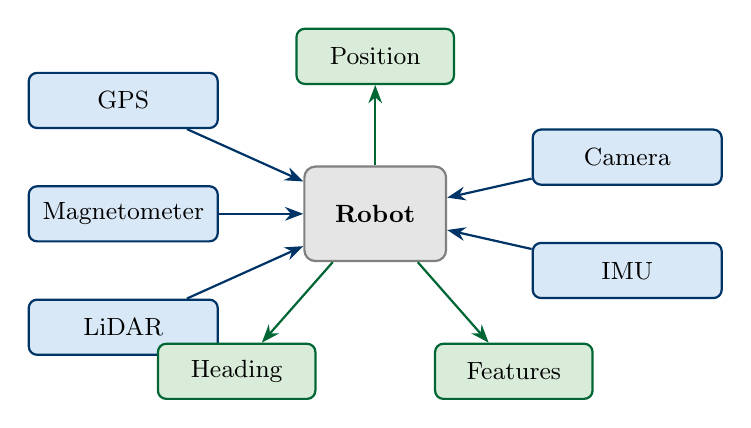
\begin{tikzpicture}[scale=0.8, >=Stealth,
        sensor/.style={draw=darkblue, thick, fill=brightblue!15, rounded corners=3pt, minimum width=2.4cm, minimum height=0.7cm, align=center, font=\small},
        info/.style={draw=darkgreen, thick, fill=accentgreen!15, rounded corners=3pt, minimum width=2cm, minimum height=0.7cm, align=center, font=\small}]
        
        % Robot
        \node[draw=gray, thick, fill=gray!20, rounded corners=4pt, minimum width=1.8cm, minimum height=1.2cm, font=\small\bfseries] (robot) at (0,0) {Robot};
        
        % Sensors
        \node[sensor] (gps) at (-4, 1.8) {GPS};
        \node[sensor] (mag) at (-4, 0) {Magnetometer};
        \node[sensor] (lidar) at (-4, -1.8) {LiDAR};
        \node[sensor] (camera) at (4, 0.9) {Camera};
        \node[sensor] (imu) at (4, -0.9) {IMU};
        
        % Information
        \node[info] (pos) at (0, 2.5) {Position};
        \node[info] (head) at (-2.2, -2.5) {Heading};
        \node[info] (feat) at (2.2, -2.5) {Features};
        
        % Arrows
        \draw[->, thick, darkblue] (gps) -- (robot);
        \draw[->, thick, darkblue] (mag) -- (robot);
        \draw[->, thick, darkblue] (lidar) -- (robot);
        \draw[->, thick, darkblue] (camera) -- (robot);
        \draw[->, thick, darkblue] (imu) -- (robot);
        
        \draw[->, thick, darkgreen] (robot) -- (pos);
        \draw[->, thick, darkgreen] (robot) -- (head);
        \draw[->, thick, darkgreen] (robot) -- (feat);
    \end{tikzpicture}
    
    \vspace{0.4cm}
    \textbf{Sensor Fusion:} Combining multiple sensors for robustness
\end{frame}

% ============================================
% SENSOR DETAILS
% ============================================
\begin{frame}{Sensor Types}
    \begin{columns}[T]
        \begin{column}{0.48\textwidth}
            \textbf{GPS:}
            \begin{itemize}
                \item Global position (lat, lon)
                \item Accuracy: 1--10 m typical
            \end{itemize}
            
            \vspace{0.4cm}
            \textbf{Magnetometer:}
            \begin{itemize}
                \item Absolute heading
                \item Subject to interference
            \end{itemize}
            
            \vspace{0.4cm}
            \textbf{IMU:}
            \begin{itemize}
                \item Accelerations, angular rates
                \item High rate, but drifts
            \end{itemize}
        \end{column}
        \begin{column}{0.48\textwidth}
            \textbf{LiDAR:}
            \begin{itemize}
                \item Point cloud data
                \item Scan matching for localization
            \end{itemize}
            
            \vspace{0.4cm}
            \textbf{Camera:}
            \begin{itemize}
                \item Feature-based localization
                \item Visual SLAM
            \end{itemize}
        \end{column}
    \end{columns}
\end{frame}

% ============================================
% GROUND TRUTH VS MEASUREMENT
% ============================================
\begin{frame}{Ground Truth vs. Measurement}
    \centering
    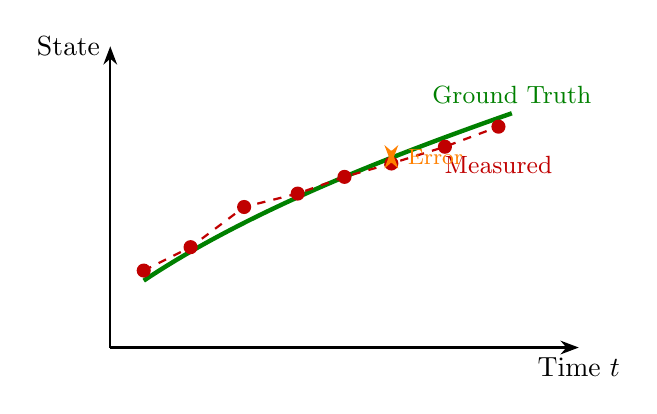
\begin{tikzpicture}[scale=0.85, >=Stealth]
        % Axes
        \draw[->, thick] (0,0) -- (7,0) node[below] {Time $t$};
        \draw[->, thick] (0,0) -- (0,4.5) node[left] {State};
        
        % Ground truth
        \draw[ultra thick, accentgreen] (0.5,1) .. controls (2,2) and (4,2.8) .. (6,3.5);
        \node[accentgreen, above, font=\small] at (6,3.5) {Ground Truth};
        
        % Measured values (noisy)
        \foreach \x/\y in {0.5/1.15, 1.2/1.5, 2/2.1, 2.8/2.3, 3.5/2.55, 4.2/2.75, 5/3.0, 5.8/3.3} {
            \fill[accentred] (\x,\y) circle (3pt);
        }
        \draw[thick, accentred, dashed] (0.5,1.15) -- (1.2,1.5) -- (2,2.1) -- (2.8,2.3) -- (3.5,2.55) -- (4.2,2.75) -- (5,3.0) -- (5.8,3.3);
        \node[accentred, below, font=\small] at (5.8,3.0) {Measured};
        
        % Error annotation
        \draw[<->, thick, accentorange] (4.2,2.75) -- (4.2,2.95);
        \node[accentorange, right, font=\footnotesize] at (4.3,2.85) {Error};
    \end{tikzpicture}
    
    \vspace{0.4cm}
    \begin{block}{Key Insight}
        There's always a gap between what's real and what sensors report.
        
        Perception = estimating and correcting this gap.
    \end{block}
\end{frame}

% ============================================
% LOCAL VS GLOBAL FRAME
% ============================================
\begin{frame}{Local Frame vs. Global Frame}
    \begin{columns}[T]
        \begin{column}{0.48\textwidth}
            \textbf{Global Frame} $\{G\}$:
            \begin{itemize}
                \item Fixed world reference
                \item Used for mapping/navigation
            \end{itemize}
            
            \vspace{0.4cm}
            \textbf{Local Frame} $\{L\}$:
            \begin{itemize}
                \item Attached to robot
                \item Moves with robot
            \end{itemize}
            
            \vspace{0.4cm}
            \textbf{Transformation:}
            \[
            \vect{p}^G = \mat{R}(\theta)\vect{p}^L + \vect{t}
            \]
        \end{column}
        \begin{column}{0.48\textwidth}
            \centering
            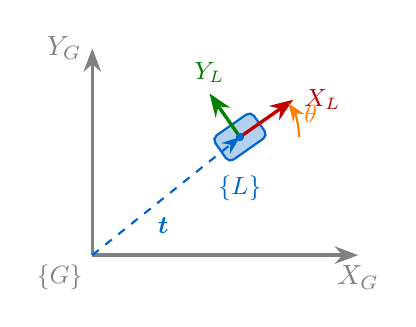
\begin{tikzpicture}[scale=0.75, >=Stealth]
                % Global frame
                \draw[->, very thick, gray] (0,0) -- (4.5,0) node[below] {$X_G$};
                \draw[->, very thick, gray] (0,0) -- (0,3.5) node[left] {$Y_G$};
                \node[gray, below left, font=\small] at (0,0) {$\{G\}$};
                
                % Robot
                \coordinate (robot) at (2.5,2);
                \begin{scope}[shift={(robot)}, rotate=35]
                    \fill[brightblue!30, draw=brightblue, thick, rounded corners=2pt] 
                        (-0.4,-0.25) rectangle (0.4,0.25);
                    
                    % Local frame
                    \draw[->, very thick, accentred] (0,0) -- (1.1,0) node[right, font=\small] {$X_L$};
                    \draw[->, very thick, accentgreen] (0,0) -- (0,0.9) node[above, font=\small] {$Y_L$};
                    \fill[brightblue] (0,0) circle (2pt);
                \end{scope}
                
                \node[brightblue, below, font=\small] at (2.5,1.5) {$\{L\}$};
                
                % Angle
                \draw[->, thick, accentorange] (3.5,2) arc (0:35:1);
                \node[accentorange, font=\small] at (3.7,2.4) {$\theta$};
                
                % Translation
                \draw[->, thick, dashed, brightblue] (0,0) -- (robot);
                \node[brightblue, below, font=\small] at (1.2,0.8) {$\vect{t}$};
            \end{tikzpicture}
        \end{column}
    \end{columns}
\end{frame}

% ============================================
% STATE SPACE WITH UNCERTAINTY
% ============================================
\begin{frame}{State-Space with Uncertainty}
    \textbf{Original (ideal) model:}
    \[
    \dot{\vect{x}} = f(\vect{x}, \vect{u})
    \]
    
    \vspace{0.4cm}
    \textbf{With uncertainties:}
    \[
    \boxed{\dot{\vect{x}} = f(\vect{x}, \vect{u}) + \vect{w}(t)}
    \]
    
    \vspace{0.3cm}
    where $\vect{w}(t)$ models:
    \begin{itemize}
        \item Process noise (unmodeled dynamics)
        \item Sensor drift
        \item Environmental disturbances
    \end{itemize}
    
    \vspace{0.4cm}
    \textbf{Measurement model:}
    \[
    \vect{y} = h(\vect{x}) + \vect{v}(t)
    \]
    
    where $\vect{v}(t)$ is measurement noise.
\end{frame}

% ============================================
% PART V: COUPLED SYSTEMS
% ============================================
\begin{frame}{}
    \vfill
    \centering
    {\Large\textbf{Part V}}
    
    \vspace{0.5cm}
    {\large Coupled Vehicle-Manipulator Systems}
    \vfill
\end{frame}

% ============================================
% SCARA ON VEHICLE
% ============================================
\begin{frame}{SCARA Manipulator on Mobile Vehicle}
    \begin{columns}[T]
        \begin{column}{0.5\textwidth}
            \textbf{System Configuration:}
            
            \vspace{0.3cm}
            \begin{itemize}
                \item Mobile base (vehicle)
                
                \vspace{0.3cm}
                \item Mounted manipulator (SCARA arm)
                
                \vspace{0.3cm}
                \item \textbf{Dynamics are coupled!}
            \end{itemize}
            
            \vspace{0.4cm}
            \begin{alertblock}{Key Insight}
                When a manipulator is mounted on a vehicle, their dynamics are \textbf{not independent}.
            \end{alertblock}
        \end{column}
        \begin{column}{0.47\textwidth}
            \centering
            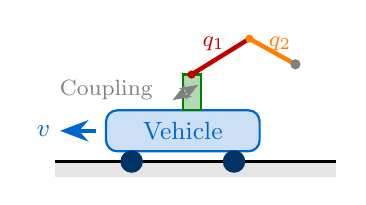
\begin{tikzpicture}[scale=0.65, >=Stealth]
                % Ground
                \fill[gray!20] (-0.5,-0.3) rectangle (5,0);
                \draw[thick] (-0.5,0) -- (5,0);
                
                % Vehicle
                \fill[brightblue!20, draw=brightblue, thick, rounded corners=4pt] 
                    (0.5,0.2) rectangle (3.5,1);
                
                % Wheels
                \fill[darkblue] (1,0) circle (0.22);
                \fill[darkblue] (3,0) circle (0.22);
                
                \node[brightblue, font=\small] at (2,0.6) {Vehicle};
                
                % Arm base
                \fill[accentgreen!30, draw=accentgreen, thick] (2,1) rectangle (2.35,1.7);
                
                % Link 1
                \draw[ultra thick, accentred] (2.17,1.7) -- (3.3,2.4);
                \fill[accentred] (2.17,1.7) circle (0.08);
                
                % Link 2
                \draw[ultra thick, accentorange] (3.3,2.4) -- (4.2,1.9);
                \fill[accentorange] (3.3,2.4) circle (0.08);
                
                % End effector
                \fill[gray] (4.2,1.9) circle (0.1);
                
                % Joint labels
                \node[accentred, font=\footnotesize] at (2.6,2.3) {$q_1$};
                \node[accentorange, font=\footnotesize] at (3.9,2.3) {$q_2$};
                
                % Vehicle motion
                \draw[->, ultra thick, brightblue] (0.3,0.6) -- (-0.4,0.6);
                \node[brightblue, left, font=\small] at (-0.4,0.6) {$v$};
                
                % Coupling
                \draw[<->, thick, dashed, gray] (1.8,1.2) -- (2.3,1.5);
                \node[gray, left, font=\footnotesize] at (1.6,1.4) {Coupling};
            \end{tikzpicture}
        \end{column}
    \end{columns}
\end{frame}

% ============================================
% ACTUATOR DYNAMICS
% ============================================
\begin{frame}{Actuator Dynamics (SCARA Arm)}
    \textbf{Manipulator dynamics:}
    \[
    \boxed{\mat{M}_a(\vect{q}_a)\ddot{\vect{q}}_a + \mat{C}_a(\vect{q}_a, \dot{\vect{q}}_a)\dot{\vect{q}}_a + \vect{G}_a(\vect{q}_a) = \vect{\tau}_a}
    \]
    
    \vspace{0.5cm}
    \begin{columns}[T]
        \begin{column}{0.48\textwidth}
            \begin{itemize}
                \item $\mat{M}_a$: Inertia of arm
                
                \vspace{0.3cm}
                \item $\mat{C}_a$: Coriolis/centrifugal
                
                \vspace{0.3cm}
                \item $\vect{G}_a$: Gravity of arm
            \end{itemize}
        \end{column}
        \begin{column}{0.48\textwidth}
            \begin{itemize}
                \item $\vect{q}_a$: Joint angles
                
                \vspace{0.3cm}
                \item $\vect{\tau}_a$: Joint torques
            \end{itemize}
        \end{column}
    \end{columns}
\end{frame}

% ============================================
% VEHICLE DYNAMICS
% ============================================
\begin{frame}{Vehicle Dynamics}
    \textbf{Mobile base dynamics:}
    \[
    \boxed{\mat{M}_v(\vect{q}_v)\ddot{\vect{q}}_v + \mat{C}_v(\vect{q}_v, \dot{\vect{q}}_v)\dot{\vect{q}}_v + \vect{G}_v(\vect{q}_v) = \vect{\tau}_v}
    \]
    
    \vspace{0.5cm}
    \begin{columns}[T]
        \begin{column}{0.48\textwidth}
            \begin{itemize}
                \item $\mat{M}_v$: Inertia of vehicle
                
                \vspace{0.3cm}
                \item $\mat{C}_v$: Coriolis/centrifugal
                
                \vspace{0.3cm}
                \item $\vect{G}_v$: Gravitational effects
            \end{itemize}
        \end{column}
        \begin{column}{0.48\textwidth}
            \begin{itemize}
                \item $\vect{q}_v$: Vehicle config $(x, y, \theta)$
                
                \vspace{0.3cm}
                \item $\vect{\tau}_v$: Driving forces/torques
            \end{itemize}
        \end{column}
    \end{columns}
\end{frame}

% ============================================
% COMBINED SYSTEM
% ============================================
\begin{frame}{Combined System Dynamics}
    \textbf{Full state vector:}
    \[
    \vect{q} = \begin{bmatrix} \vect{q}_v \\ \vect{q}_a \end{bmatrix}
    \]
    
    \vspace{0.4cm}
    \textbf{Unified dynamics:}
    \[
    \boxed{\mat{M}(\vect{q})\ddot{\vect{q}} + \mat{C}(\vect{q}, \dot{\vect{q}})\dot{\vect{q}} + \vect{G}(\vect{q}) = \vect{\tau}}
    \]
    
    \vspace{0.3cm}
    where $\vect{\tau} = \begin{bmatrix} \vect{\tau}_v \\ \vect{\tau}_a \end{bmatrix}$
    
    \vspace{0.4cm}
    \begin{block}{Important}
        Cannot write as two independent systems --- coupling terms arise from interaction.
    \end{block}
\end{frame}

% ============================================
% BLOCK MATRIX
% ============================================
\begin{frame}{Block Matrix Structure}
    \textbf{Block matrix form:}
    \[
    \mat{M}(\vect{q}) = \begin{bmatrix} \mat{M}_{vv} & \mat{M}_{va} \\ \mat{M}_{av} & \mat{M}_{aa} \end{bmatrix}
    \]
    
    \vspace{0.4cm}
    \begin{columns}[T]
        \begin{column}{0.45\textwidth}
            \centering
            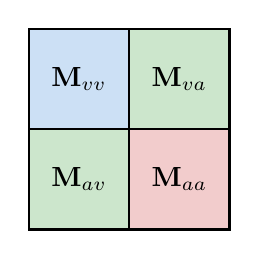
\begin{tikzpicture}[scale=0.85]
                % Matrix
                \fill[brightblue!20] (0,1.5) rectangle (1.5,3);
                \fill[accentgreen!20] (1.5,1.5) rectangle (3,3);
                \fill[accentgreen!20] (0,0) rectangle (1.5,1.5);
                \fill[accentred!20] (1.5,0) rectangle (3,1.5);
                
                \draw[thick] (0,0) rectangle (3,3);
                \draw[thick] (1.5,0) -- (1.5,3);
                \draw[thick] (0,1.5) -- (3,1.5);
                
                \node at (0.75,2.25) {$\mat{M}_{vv}$};
                \node at (2.25,2.25) {$\mat{M}_{va}$};
                \node at (0.75,0.75) {$\mat{M}_{av}$};
                \node at (2.25,0.75) {$\mat{M}_{aa}$};
            \end{tikzpicture}
        \end{column}
        \begin{column}{0.5\textwidth}
            \begin{itemize}
                \item \textcolor{brightblue}{$\mat{M}_{vv}$}: Vehicle inertia
                
                \vspace{0.3cm}
                \item \textcolor{accentred}{$\mat{M}_{aa}$}: Arm inertia
                
                \vspace{0.3cm}
                \item \textcolor{accentgreen}{$\mat{M}_{va}, \mat{M}_{av}$}: \textbf{Coupling}
            \end{itemize}
            
            \vspace{0.3cm}
            {\small $\mat{M}_{av} = \mat{M}_{va}^T$ (symmetry)}
        \end{column}
    \end{columns}
\end{frame}

% ============================================
% COUPLING EXPLANATION
% ============================================
\begin{frame}{Understanding the Coupling}
    \textbf{Physical interpretation:}
    
    \vspace{0.4cm}
    \begin{itemize}
        \item $\mat{M}_{va}$: How manipulator motion affects vehicle
        
        \vspace{0.3cm}
        \item $\mat{M}_{av}$: How vehicle motion affects manipulator
    \end{itemize}
    
    \vspace{0.5cm}
    \begin{exampleblock}{Example}
        When the arm swings, it creates reaction forces on the vehicle.
        
        When the vehicle accelerates, the arm experiences inertial forces.
    \end{exampleblock}
    
    \vspace{0.4cm}
    \textbf{Controller must account for these coupling effects!}
\end{frame}

% ============================================
% MECANUM EXTENSION
% ============================================
\begin{frame}{Extension: Mecanum/Omnidirectional Vehicles}
    \textbf{For mecanum wheel robots:}
    
    \vspace{0.4cm}
    \begin{itemize}
        \item 3 or 4 mecanum wheels
        
        \vspace{0.3cm}
        \item Extra degrees of freedom (holonomic)
        
        \vspace{0.3cm}
        \item Vehicle inertia matrix increases: $3 \times 3 \to 4 \times 4$
    \end{itemize}
    
    \vspace{0.5cm}
    \textbf{Same block structure applies:}
    \[
    \mat{M} = \begin{bmatrix} \mat{M}_{vv}^{n \times n} & \mat{M}_{va} \\ \mat{M}_{av} & \mat{M}_{aa}^{m \times m} \end{bmatrix}
    \]
    
    \vspace{0.3cm}
    Only the dimensions change --- the framework generalizes.
\end{frame}

% ============================================
% KEY POINTS COUPLED
% ============================================
\begin{frame}{Key Points: Coupled Systems}
    \begin{block}{Summary}
        \begin{itemize}
            \item Vehicle and manipulator dynamics are \textbf{not independent}
            
            \vspace{0.3cm}
            \item Must model \textbf{coupling} between them
            
            \vspace{0.3cm}
            \item Block matrix structure reveals interactions
        \end{itemize}
    \end{block}
    
    \vspace{0.4cm}
    \textbf{Framework generalizes to:}
    \begin{itemize}
        \item Any manipulator-on-mobile-base system
        \item Robotic arms on AGVs
        \item Dual-arm mobile manipulators
    \end{itemize}
\end{frame}

% ============================================
% PART VI: TRANSFORMATIONS
% ============================================
\begin{frame}{}
    \vfill
    \centering
    {\Large\textbf{Part VI}}
    
    \vspace{0.5cm}
    {\large Coordinate Transformations}
    \vfill
\end{frame}

% ============================================
% LOOK AHEAD POINT
% ============================================
\begin{frame}{Look-Ahead Point Control}
    \begin{columns}[T]
        \begin{column}{0.48\textwidth}
            \textbf{Define point $Y$ ahead of robot:}
            \[
            \vect{Y} = \begin{bmatrix} x + L\cos\theta \\ y + L\sin\theta \end{bmatrix}
            \]
            
            \vspace{0.4cm}
            \textbf{Velocity of point $Y$:}
            \[
            \dot{\vect{Y}} = \begin{bmatrix} v\cos\theta - L\omega\sin\theta \\ v\sin\theta + L\omega\cos\theta \end{bmatrix}
            \]
        \end{column}
        \begin{column}{0.48\textwidth}
            \centering
            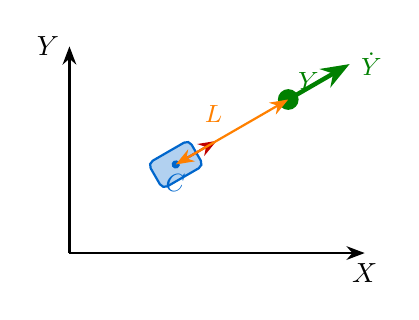
\begin{tikzpicture}[scale=0.75, >=Stealth]
                % Axes
                \draw[->, thick] (0,0) -- (5,0) node[below] {$X$};
                \draw[->, thick] (0,0) -- (0,3.5) node[left] {$Y$};
                
                % Robot
                \coordinate (robot) at (1.8,1.5);
                \begin{scope}[shift={(robot)}, rotate=30]
                    \fill[brightblue!30, draw=brightblue, thick, rounded corners=2pt] 
                        (-0.4,-0.25) rectangle (0.4,0.25);
                    \draw[->, thick, accentred] (0,0) -- (0.8,0);
                    \fill[brightblue] (0,0) circle (2pt);
                \end{scope}
                
                % Look-ahead point
                \coordinate (Y) at ($(robot) + (30:2.2)$);
                \fill[accentgreen] (Y) circle (5pt);
                \node[accentgreen, above right, font=\small] at (Y) {$Y$};
                
                % Distance L
                \draw[<->, thick, accentorange] (robot) -- (Y);
                \node[accentorange, above left, font=\small] at ($(robot)!0.5!(Y)$) {$L$};
                
                % Velocity at Y
                \draw[->, ultra thick, accentgreen] (Y) -- ++(30:1.2) node[right, font=\small] {$\dot{Y}$};
                
                % Robot label
                \node[brightblue, below, font=\small] at (robot) {$C$};
            \end{tikzpicture}
        \end{column}
    \end{columns}
\end{frame}

% ============================================
% JACOBIAN
% ============================================
\begin{frame}{Jacobian Transformation}
    \textbf{Matrix form:}
    \[
    \dot{\vect{Y}} = \mat{J}(\theta) \begin{bmatrix} v \\ \omega \end{bmatrix}
    \]
    
    \vspace{0.3cm}
    where the Jacobian is:
    \[
    \mat{J}(\theta) = \begin{bmatrix} \cos\theta & -L\sin\theta \\ \sin\theta & L\cos\theta \end{bmatrix}
    \]
    
    \vspace{0.4cm}
    \textbf{Key property:}
    \[
    \det(\mat{J}) = L\cos^2\theta + L\sin^2\theta = L \neq 0
    \]
    
    \vspace{0.3cm}
    The Jacobian is always invertible for $L > 0$!
\end{frame}

% ============================================
% INVERSE JACOBIAN
% ============================================
\begin{frame}{Inverse Jacobian}
    \textbf{Inverse relation:}
    \[
    \begin{bmatrix} v \\ \omega \end{bmatrix} = \mat{J}^{-1}(\theta)\,\dot{\vect{Y}}
    \]
    
    \vspace{0.4cm}
    \[
    \mat{J}^{-1}(\theta) = \frac{1}{L}\begin{bmatrix} L\cos\theta & L\sin\theta \\ -\sin\theta & \cos\theta \end{bmatrix}
    \]
    
    \vspace{0.5cm}
    \begin{block}{Control Advantage}
        Control the look-ahead point $Y$ instead of robot center.
        
        Makes trajectory tracking simpler (feedback linearization).
    \end{block}
\end{frame}

% ============================================
% TRANSFORMED DYNAMICS
% ============================================
\begin{frame}{Transformed Dynamics}
    \textbf{Define transformed (barred) matrices:}
    
    \vspace{0.3cm}
    \[
    \bar{\mat{M}} = (\bar{\mat{J}}^{-1})^T \mat{M} \bar{\mat{J}}^{-1}
    \]
    
    \vspace{0.2cm}
    \[
    \bar{\mat{C}} = (\bar{\mat{J}}^{-1})^T \left( \mat{C} - \mat{M}\bar{\mat{J}}^{-1}\dot{\bar{\mat{J}}} \right) \bar{\mat{J}}^{-1}
    \]
    
    \vspace{0.4cm}
    \textbf{Final dynamics at point $Y$:}
    \[
    \boxed{\bar{\mat{M}}\ddot{\vect{Y}} + \bar{\mat{C}}\dot{\vect{Y}} + \bar{\vect{G}} = \bar{\mat{B}}\vect{F}}
    \]
    
    \vspace{0.3cm}
    This enables direct control of the look-ahead point position.
\end{frame}

% ============================================
% PART VII: SWERVE DRIVE
% ============================================
\begin{frame}{}
    \vfill
    \centering
    {\Large\textbf{Part VII}}
    
    \vspace{0.5cm}
    {\large 4-Independent Wheel Drive (Swerve)}
    \vfill
\end{frame}

% ============================================
% SWERVE CONFIG
% ============================================
\begin{frame}{Swerve Drive: Configuration}
    \begin{columns}[T]
        \begin{column}{0.48\textwidth}
            \textbf{Configuration:}
            
            \vspace{0.3cm}
            \begin{itemize}
                \item 4 independently controlled wheels
                
                \vspace{0.3cm}
                \item Each wheel has 2 actuations:
                \begin{itemize}
                    \item Steering angle $\delta_i$
                    \item Driving force $F_i$
                \end{itemize}
                
                \vspace{0.3cm}
                \item Total: 8 control inputs
            \end{itemize}
            
            \vspace{0.4cm}
            \textbf{Advantages:}
            \begin{itemize}
                \item Holonomic motion
                \item High maneuverability
            \end{itemize}
        \end{column}
        \begin{column}{0.48\textwidth}
            \centering
            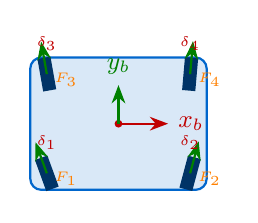
\begin{tikzpicture}[scale=0.7, >=Stealth]
                % Vehicle body
                \fill[brightblue!15, draw=brightblue, thick, rounded corners=4pt] 
                    (-1.6,-1.2) rectangle (1.6,1.2);
                
                % Wheels with steering
                \foreach \x/\y/\angle/\num in {-1.3/-0.9/20/1, 1.3/-0.9/-15/2, -1.3/0.9/10/3, 1.3/0.9/-5/4} {
                    \begin{scope}[shift={(\x,\y)}, rotate=\angle]
                        \fill[darkblue] (-0.12,-0.3) rectangle (0.12,0.3);
                        \draw[->, thick, accentgreen] (0,0) -- (0,0.6);
                    \end{scope}
                    \node[accentred, font=\tiny] at (\x,\y+0.55) {$\delta_\num$};
                    \node[accentorange, font=\tiny] at (\x+0.35,\y-0.1) {$F_\num$};
                }
                
                % Center
                \fill[accentred] (0,0) circle (2pt);
                
                % Body frame
                \draw[->, thick, accentred] (0,0) -- (0.9,0) node[right, font=\small] {$x_b$};
                \draw[->, thick, accentgreen] (0,0) -- (0,0.7) node[above, font=\small] {$y_b$};
            \end{tikzpicture}
        \end{column}
    \end{columns}
\end{frame}

% ============================================
% FORCE BALANCE X
% ============================================
\begin{frame}{Force Balance: $x$-Direction}
    \textbf{Force balance in $x$:}
    \[
    m\ddot{x} = \sum_{i=1}^{4} F_i \cos(\theta + \delta_i)
    \]
    
    \vspace{0.4cm}
    \centering
    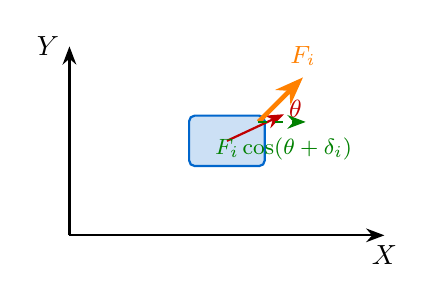
\begin{tikzpicture}[scale=0.8, >=Stealth]
        % Axes
        \draw[->, thick] (0,0) -- (5,0) node[below] {$X$};
        \draw[->, thick] (0,0) -- (0,3) node[left] {$Y$};
        
        % Robot
        \coordinate (robot) at (2.5,1.5);
        \fill[brightblue!20, draw=brightblue, thick, rounded corners=2pt] 
            ($(robot) + (-0.6,-0.4)$) rectangle ($(robot) + (0.6,0.4)$);
        
        % Robot heading
        \draw[->, thick, accentred] (robot) -- ++(25:1);
        \node[accentred, font=\small] at ($(robot) + (25:1.2)$) {$\theta$};
        
        % One wheel force
        \coordinate (wheel) at ($(robot) + (0.5,0.3)$);
        \draw[->, ultra thick, accentorange] (wheel) -- ++(45:1) node[above, font=\small] {$F_i$};
        \draw[->, thick, accentgreen, dashed] (wheel) -- ++(0:0.75);
        \node[accentgreen, below, font=\footnotesize] at ($(wheel) + (0.4,-0.1)$) {$F_i\cos(\theta+\delta_i)$};
    \end{tikzpicture}
\end{frame}

% ============================================
% FORCE BALANCE Y
% ============================================
\begin{frame}{Force Balance: $y$-Direction}
    \textbf{Force balance in $y$:}
    \[
    m\ddot{y} = \sum_{i=1}^{4} F_i \sin(\theta + \delta_i)
    \]
    
    \vspace{0.5cm}
    Each wheel contributes:
    \begin{itemize}
        \item $F_i\cos(\theta + \delta_i)$ in global $X$
        
        \vspace{0.3cm}
        \item $F_i\sin(\theta + \delta_i)$ in global $Y$
    \end{itemize}
    
    \vspace{0.4cm}
    Robot motion = combined effect of all 4 wheels.
\end{frame}

% ============================================
% TORQUE BALANCE
% ============================================
\begin{frame}{Torque Balance: Yaw Motion}
    \textbf{Moment balance about center of mass:}
    \[
    I_{zz}\ddot{\theta} = \sum_{i=1}^{4} \vect{r}_i \times \vect{F}_i
    \]
    
    \vspace{0.4cm}
    \textbf{Expanded:}
    \[
    I_{zz}\ddot{\theta} = \sum_{i=1}^{4} \left[ x_i F_i\sin(\theta + \delta_i) - y_i F_i\cos(\theta + \delta_i) \right]
    \]
    
    \vspace{0.3cm}
    where $(x_i, y_i)$ is wheel $i$ position relative to center.
    
    \vspace{0.4cm}
    \begin{block}{Control Allocation}
        Given desired $(\ddot{x}, \ddot{y}, \ddot{\theta})$, solve for $F_i$ and $\delta_i$.
        
        Over-actuated system with redundancy.
    \end{block}
\end{frame}

% ============================================
% SWERVE MATRIX FORM
% ============================================
\begin{frame}{Swerve Drive: Matrix Form}
    \textbf{State:} $\vect{q} = [x, y, \theta]^T$
    
    \vspace{0.4cm}
    \textbf{Dynamics:}
    \[
    \mat{M}\ddot{\vect{q}} = \mat{B}(\vect{q}, \vect{\delta})\vect{F}
    \]
    
    \vspace{0.3cm}
    where:
    \[
    \mat{M} = \begin{bmatrix} m & 0 & 0 \\ 0 & m & 0 \\ 0 & 0 & I_{zz} \end{bmatrix}
    \]
    
    \vspace{0.3cm}
    \[
    \mat{B} = \begin{bmatrix} 
        \cos(\theta+\delta_1) & \cos(\theta+\delta_2) & \cos(\theta+\delta_3) & \cos(\theta+\delta_4) \\
        \sin(\theta+\delta_1) & \sin(\theta+\delta_2) & \sin(\theta+\delta_3) & \sin(\theta+\delta_4) \\
        r_1^{\perp} & r_2^{\perp} & r_3^{\perp} & r_4^{\perp}
    \end{bmatrix}
    \]
\end{frame}

% ============================================
% HOMEWORK
% ============================================
\begin{frame}{Homework: Simulation \& Validation}
    \textbf{Numerical integration (Euler method):}
    \[
    \vect{x}(t + \Delta t) = \vect{x}(t) + \dot{\vect{x}}(t) \cdot \Delta t
    \]
    
    \vspace{0.4cm}
    \textbf{Simulation parameters:}
    \begin{itemize}
        \item Duration: $T = 10$ s
        \item Step size: $\Delta t = 0.01$ s
        \item Tools: MATLAB, Simulink, or Python
    \end{itemize}
    
    \vspace{0.4cm}
    \textbf{Goal:}
    \begin{itemize}
        \item Verify simulated path matches expectations
        \item Test: straight line, circular arc, figure-8
    \end{itemize}
\end{frame}

% ============================================
% SUMMARY
% ============================================
\begin{frame}{Lecture Summary}
    \begin{columns}[T]
        \begin{column}{0.48\textwidth}
            \textbf{Dynamics:}
            \begin{itemize}
                \item Euler-Lagrange formulation
                \item Balancing robot example
                \item Matrix form: $\mat{M}\ddot{\vect{q}} + \mat{C}\dot{\vect{q}} + \vect{G} = \vect{\tau}$
            \end{itemize}
            
            \vspace{0.4cm}
            \textbf{Perception:}
            \begin{itemize}
                \item Sensor types
                \item Ground truth vs. measurement
                \item Uncertainty modeling
            \end{itemize}
        \end{column}
        \begin{column}{0.48\textwidth}
            \textbf{Coupled Systems:}
            \begin{itemize}
                \item Vehicle-manipulator coupling
                \item Block matrix structure
            \end{itemize}
            
            \vspace{0.4cm}
            \textbf{Transformations:}
            \begin{itemize}
                \item Look-ahead point control
                \item Jacobian transformations
                \item Swerve drive dynamics
            \end{itemize}
        \end{column}
    \end{columns}
\end{frame}

% ============================================
% END SLIDE
% ============================================
{
\setbeamertemplate{footline}{}
\begin{frame}[plain]
    \vfill
    \centering
    {\Large\textbf{End of Lecture 3}}
    
    \vspace{1cm}
    {\large Control \& Perception Fundamentals}
    
    \vspace{1.5cm}
    {\Large Questions?}
    \vfill
\end{frame}
}

\end{document}
